\documentclass[border=3pt]{standalone}
\usepackage{circuitikz}
\usetikzlibrary{positioning}
\ctikzset{logic ports=ieee, logic ports/scale=0.9}
\begin{document}
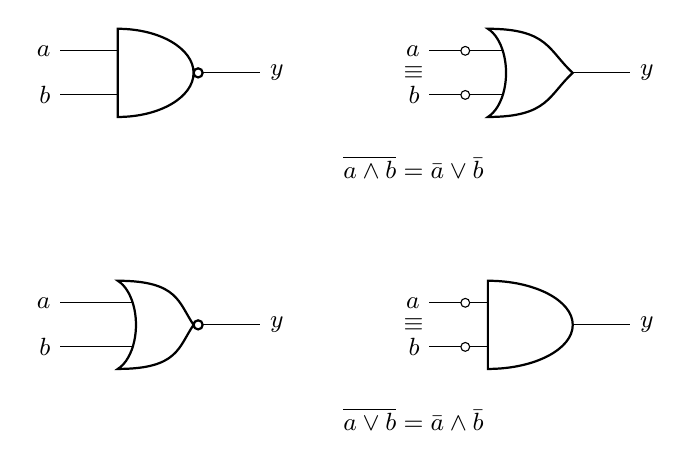
\begin{tikzpicture}[font=\sffamily\small]
  % NAND = OR with bubbled inputs
  \node[nand port] (n1) at (0,0) {};
  \draw (n1.in 1) -- ++(-0.5,0) node[left]{$a$};
  \draw (n1.in 2) -- ++(-0.5,0) node[left]{$b$};
  \draw (n1.out) -- ++(0.5,0) node[right]{$y$};
  \node at (2.6,0) {$\equiv$};
  \node[or port] (n2) at (4.7,0) {};
  \node[ocirc, anchor=east] (b1) at (n2.in 1) {};
  \node[ocirc, anchor=east] (b2) at (n2.in 2) {};
  \draw (b1.west) -- ++(-0.4,0) node[left]{$a$};
  \draw (b2.west) -- ++(-0.4,0) node[left]{$b$};
  \draw (n2.out) -- ++(0.5,0) node[right]{$y$};
  \node at (2.6,-1.2) {$\overline{a \land b} = \bar{a} \lor \bar{b}$};
  % NOR = AND with bubbled inputs
  \node[nor port] (n3) at (0,-3.2) {};
  \draw (n3.in 1) -- ++(-0.5,0) node[left]{$a$};
  \draw (n3.in 2) -- ++(-0.5,0) node[left]{$b$};
  \draw (n3.out) -- ++(0.5,0) node[right]{$y$};
  \node at (2.6,-3.2) {$\equiv$};
  \node[and port] (n4) at (4.7,-3.2) {};
  \node[ocirc, anchor=east] (b3) at (n4.in 1) {};
  \node[ocirc, anchor=east] (b4) at (n4.in 2) {};
  \draw (b3.west) -- ++(-0.4,0) node[left]{$a$};
  \draw (b4.west) -- ++(-0.4,0) node[left]{$b$};
  \draw (n4.out) -- ++(0.5,0) node[right]{$y$};
  \node at (2.6,-4.4) {$\overline{a \lor b} = \bar{a} \land \bar{b}$};
\end{tikzpicture}
\end{document}
